\documentclass{jsarticle}

\usepackage{amssymb}
\usepackage{graphicx}
\usepackage[dvipdfmx]{color}
\usepackage{here}
\usepackage{tabularx}
\usepackage{amsmath}
\usepackage{url}
\usepackage[hang,small,bf]{caption}
\usepackage[subrefformat=parens]{subcaption}
\usepackage{tikz}
\usepackage{siunitx}
\usepackage{bm}
\usepackage[top=15truemm,bottom=20truemm,left=20truemm,right=20truemm]{geometry}
\usetikzlibrary{shapes.geometric}
\usetikzlibrary {shapes.misc}
\usetikzlibrary{positioning}
\captionsetup{compatibility=false}
 
\begin{document}

日付:4/12,13

\section*{Ex1.6}
Sec1.3の最後で説明したロケット制御問題の2つの場合について線形計画法を用いて定式化せよ。\\

前提:\\
まっすぐな経路に沿って移動するロケットについて考える。\\
$x_t,v_t,a_t$はそれぞれ時間$t$でのロケットの位置、速度、加速度。\\
時間は離散的に考え、$x_{t+1}=x_t+v_t,v_{t+1}=v_t+a_t$が成り立つ。\\
$a_t$は私たちの制御下にあると仮定。\\
ロケットは最初原点で静止、$x_0=0,v_0=0$と仮定。\\
加速度の大きさ$|a_t|$は時間$t$での燃料消費率に比例すると仮定。\\
$T$時間後、「ソフトに着陸」つまり、$x_T=1,v_T=0$させる。\\

case1:\\
総燃料消費量、$\sum_{t=0}^{T-1}|a_t|$が最小になるように考える。

\begin{equation}
\begin{array}{cc}
\text { minimize } & \sum_{t=0}^{T-1}z_t \\
\text { subject to } & a_t\leq z_t \\
& -a_t\leq z_t\\
&x_{t+1}=x_t+v_t\\
&v_{t+1}=v_t+a_t\\
&x_0=0\\
&v_0=0\\
&x_T=1\\
&v_T=0\\
&(t=0,1,...,T-1)
\end{array}
\end{equation}

$|a_t|=z_t$とおき、上2つの条件を追加した。\\
case2:\\
必要最大燃料、$max_t|a_t|$最小になるように考える。
\begin{equation}
\begin{array}{cc}
\text { minimize } & z \\
\text { subject to } & a_t\leq z \\
& -a_t\leq z\\
&x_{t+1}=x_t+v_t\\
&v_{t+1}=v_t+a_t\\
&x_0=0\\
&v_0=0\\
&x_T=1\\
&v_T=0\\
&(t=0,1,...,T-1)
\end{array}
\end{equation}
$max_t|a_t|=z$とおき、上2つの条件を追加した。

\newpage

\section*{Ex1.12(Chebychev center)}

線形不等式制約によって記述された集合Pを考える。つまり、$P=\{\bm{x}\in \mathbb{R}^n|\bm{a}'_i\bm{x}\leq b_i,i = 1,...,m\}$。 中心が$\bm{y}$で半径が$r$の球は、$\bm{y}$からユークリッド距離$r$内にあるすべての点のセットとして定義されます。 集合$P$内に完全に含まれる、可能な限り最大の半径を持つ球を見つけたい。(このような球の中心は$P$のチェビチェフ中心と呼ばれる)。この問題を線形計画法を用いて定式化せよ。

\begin{equation}
\begin{array}{cc}
\text { miximize } & r \\
\text { subject to } & \bm{a}'_i\bm{y}+r||\bm{a}_i||\leq b_i\\
&(i=1,...,m)
\end{array}
\end{equation}
\\
まず、線形不等式制約によって記述された集合$P$とは多面体である。簡単のため2次元的に記述した下の図でみると、5角形の内部が集合$P$である。半径$r$を最大にしたい。そこで、円の中心からどれくらい離れているかを表すベクトル$\bm{u}$を考える。$|\bm{u}|\leq r$である。
集合$P$の定義から考えると、
\begin{equation}
\bm{a}'_i(\bm{y}+\bm{u})\leq b_i
\end{equation}
が成り立たなければならない。これは、
\begin{equation}
max_{\bm{u}}\{\bm{a}'_i(\bm{y}+\bm{u})\mid ||\bm{u}||\leq r\}\leq b_i
\end{equation}
と同義であるため、上の解答が導かれる。

\begin{figure}[H]
  \centering
  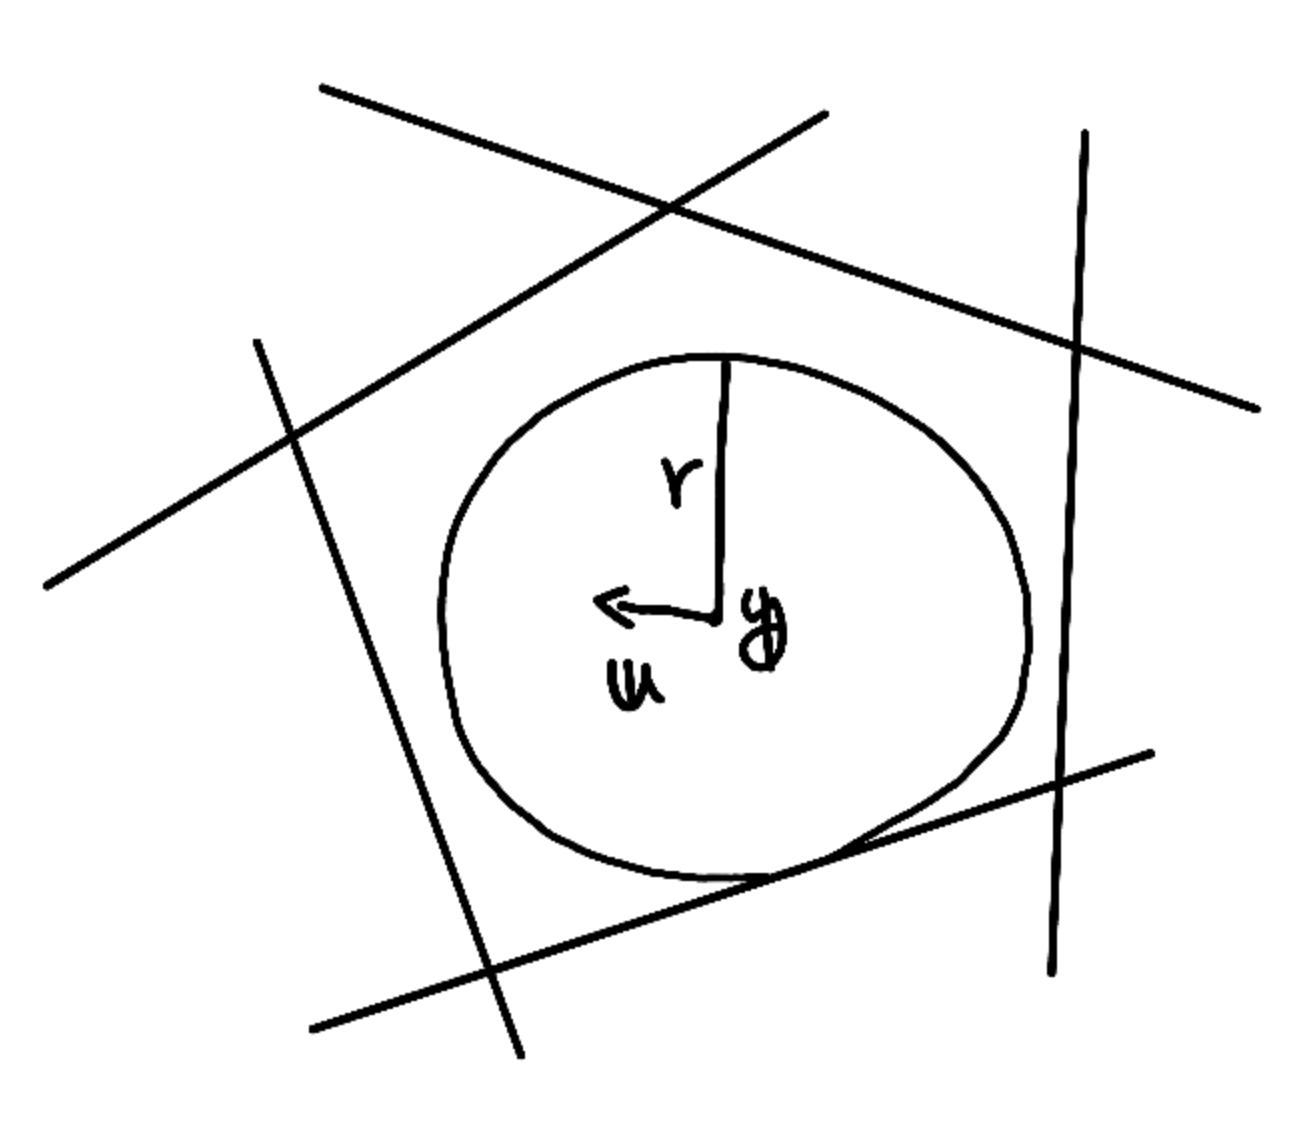
\includegraphics[width=5cm]{center.png}
  \caption{2次元での例}
\end{figure}


\end{document}